
% \section{\textls[-40]{\solution: SELF-SUPERVISED ENTITY ALIGNMENT}}
\section{{SELF-SUPERVISED ENTITY ALIGNMENT}} \label{sec:model}
%\yukuo{Maybe use this section name as paper title? SelfKG: Self-supervised entity alignment}


In this section, we discuss the role that the supervision plays in entity alignment and then present the strategies that can help align entities without label supervision. 
To this end, we present the \solution framework for self-supervised entity alignment across KGs. 


\subsection{The \solution Framework} \label{sec:architecture}

%\vpara{\solution.}
To enable learning without label information, the main goal of \solution is to design a self-supervised  objective that can guide its learning process. 
To achieve this, we propose the concept of \textit{relative similarity metric} (Cf. Section ~\ref{sec:rsm}) between entities across two KGs. 
To further improve the self-supervised optimization of \solution, we introduce the techniques of \textit{self-negative sampling} (Cf. Section ~\ref{sec:sns}) and \textit{multiple negative queues} (Cf. Section ~\ref{sec:mnq}). 


%Figure \ref{fig:modelflow} illustrates the training process of \solution. 
%\yx{to describe the model figure}




Next, we introduce the initialization of entity embeddings in \solution, which is largely built upon existing techniques, including the uni-space learning and GNN based neighborhood aggregator. 

\vpara{Uni-space learning.} 
The idea of uni-space learning has been adopted by recent (semi-) supervised entity alignment techniques~\cite{{MTransE,GCN-Align,CEAFF,tang2019bert-int,wu2019relation}}. 
Herein, we present how we leverage it for supporting \solution's self-supervised learning setting. 


%The measure of similarity is required to be in the same space.
Straightforwardly, embedding entities from different KGs into a uni-space can greatly benefit the alignment task. 
With labeled entity pairs, it is natural to leverage supervision to align different spaces into one, e.g., merging aligned entities for training ~\cite{hao2016joint}, or learning projection matrices with abundant training labels to project entities from different embedding spaces into a uni-space~\cite{MTransE,JAPE}. 

In terms of multi-lingual datasets (e.g., DBP15K), the issue is more challenging. 
%Most existing methods would either train projection matrices by supervision~\cite{GCN-Align} or leverage Google Translate to translate the dataset into English to use Glove embeddings~\cite{wu2019relation,fey2020deep,wu2019jointly}.
Thanks to the pre-trained language models~\cite{han2021pre}, high-quality multi-lingual initial embeddings are now available. For example, the multi-lingual BERT has been used in recent work~\cite{zhang2019multi,tang2019bert-int}. In \solution, we adopt LaBSE~\cite{feng2020language}---a state-of-the-art multi-lingual pre-trained language model trained on 109 different languages---for embedding different knowledge graphs into a uni-space. 




\vpara{Neighborhood aggregator. \label{na}}
To further improve the entity embeddings, 
the neighborhood aggregation is used to aggregate neighbor entities' information to the center entity~\cite{GCN-Align,xu2019cross-lingual}. 
In this work, we directly use a single-head graph attention network~\cite{velivckovic2017graph} with one layer to aggregate pre-trained embeddings of one-hop neighbors.

Note that leveraging multi-hop graph structures has been recently explored for the problem of entity alignment. 
Though some studies~\cite{fey2020deep,wu2019relation,GCN-Align} claim that they benefit from multi-hop neighbors, other works~\cite{xu2019cross-lingual,zhang2018mego2vec} argue that one-hop neighbors provides enough information for most situations. 
In our ablation study (Cf. Section ~\ref{sec:ablation}), we find that the multi-hop information actually harms the performance of \solution, which is probably resulted from the distant neighbor noises that may be unignorable in a self-supervised setting. 
%In addition, it is also a problem that whether we should utilize relation information. 
%Intuitively it would be helpful, but the issue is that different knowledge graphs often have very different schema and can introduce difficulty into the implementation.
Therefore, to demonstrate the minimum requirement of self-supervision for entity alignment, we only involve one-hop neighbor entities during the aggregation. %, without additional structure or relation information. 
%Specifically we employ a single-head graph attention network to collect information from 1-hop neighbors. 




\begin{figure}[t]
\centering
%\setlength{\abovecaptionskip}{-0.2mm}
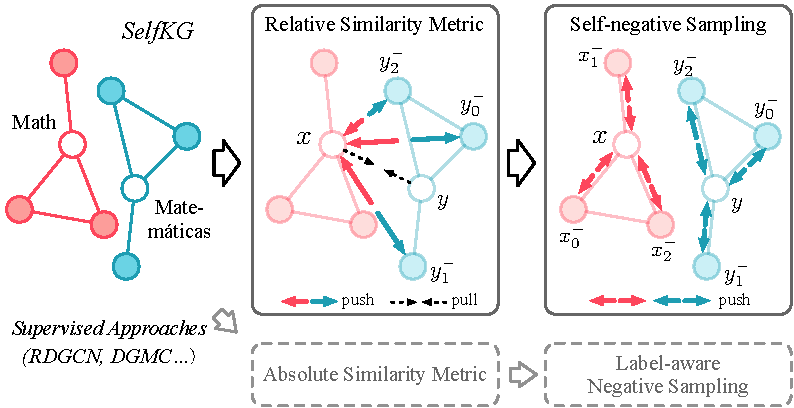
\includegraphics[width=\linewidth]{img/selfkg-new.pdf}
\caption{A conceptual comparison of \solution and supervised approaches. \textmd{\solution employs the relative similarity metric (RSM) and self-negative sampling to avoid the use of supervision.}
\label{fig:motivations}
% \textmd{
% }
}
% 
\vspace{-3mm}
\end{figure}



 
\subsection{Relative Similarity Metric}
\label{sec:rsm}

We present the self-supervised loss for entity alignment across KGs. 
First, we analyze the supervised NCE loss for entity alignment. 
Then, we introduce the relative similarity metric for avoiding labeled  pairs. 
We finally derive the self-supervised NCE for \solution. 

In representation learning, the margin loss~\cite{bordes2013translating,tang2019bert-int} and cross-entropy loss~\cite{zhang2019oag} have been widely adopted as the similarity metric. 
Without loss of generality, they can be expressed in the form of Noise Contrastive Estimation (NCE)~\cite{gutmann2010noise}. 

In the context of entity alignment, the NCE loss can be formalized as follows. 
Let $p_{\mathsf x}, p_{\mathsf y}$ be the distributions of two KGs $G_\mathrm{x}$, $G_\mathrm{y}$, and $p_{pos}$ denote the representation distribution of the positive entity pairs $(x,y)\in\mathbb{R}^n\times\mathbb{R}^n$.
%\yukuo{The format of y should be unified. $p_y$ or $p_{\mathsf y}$. } 
Given a pair of aligned entities $(x, y) \sim \distnpos$, negative samples ${\{y^-_i\}}_{i=1}^M \iidsim p_{\mathsf y}$, the temperature $\tau$, and the encoder $f$ satisfies $\|f(\cdot)\|=1$, we have the supervised NCE loss as  
\beqn{\scriptsize
\begin{aligned}
\label{eq:nce}
\mathcal{L}_{\rm NCE} &\trieq 
{- \log \frac{e^{f(x)\T f(y) / \tau}}{e^{f(x)\T f(y) / \tau} + \sum_i e^{f(x)\T  f(y^-_i)/ \tau}}}\\
&= \underbrace{-\frac{1}{\tau}f(x)\T f(y)}_{\rm alignment} + \underbrace{\mathop{\log}(e^{f(x)\T f(y) / \tau} + \sum_ie^{f(x)\T f(y^-_i) / \tau})}_{\rm uniformity}.
\end{aligned}
}

\vspace{-0.2cm}
\noindent where the ``alignment'' term is to draw the positive pair close and the ``uniformity'' term is to push the negative pairs away. 
%\yukuo{need to explain the meaning of $\tau$}

We illustrate how this NCE loss can be further adjusted for a self-supervised setting. 
An example of ``pulling'' and ``pushing'' entity pairs in KGs can be found in Figure ~\ref{fig:motivations} (left). 
Previous studies have shown that the NCE loss has the following asymptotic properties: 

\begin{theorem}{\bf (Absolute similarity metric (ASM)~\cite{wang2020understanding})} \label{th:asm}
For a fixed $\tau > 0$, as the number of negative samples $M \rightarrow \infty$, the (normalized) contrastive loss $\mathcal{L}_{\rm NCE}$ (i.e., $\mathcal{L}_{\rm ASM}$) converges to its limit with an absolute deviation decaying in $\mathcal{O}(M^{-2/3})$. If a perfectly-uniform encoder $f$ exists, it forms the exact minimizer of the uniformity term.
\end{theorem}

\vspace{-0.2cm}

\begin{pf}
    Please refer to~\cite{wang2020understanding}. \hfill$\square$
\end{pf}

Theorem~\ref{th:asm} makes the NCE loss an absolute similarity metric that requires supervision. 
However, note that despite potential ambiguity and heterogeneity for entities in KGs, the aligned pairs should share similar semantic meanings, if not exactly the name. 
Furthermore, the pre-trained word embeddings are known to capture this semantic similarity by projecting similar entities close in the embedding space, which can thus ensure a relatively large $f(x)^Tf(y)$ in Eq.~\ref{eq:nce}, i.e., the ``alignment'' term.  

Therefore, to optimize the NCE loss, the main task is then to optimize the ``uniformity'' term in Eq.~\ref{eq:nce} rather than the ``alignment'' term. 
Considering the boundedness property of $f$, we can instantly draw an unsupervised upper bound of $\mathcal{L}_{\rm ASM}$ by as follows. 


\begin{proposition}{\bf Relative similarity metric (RSM).} \label{th:rsm}
For a fixed $\tau > 0$ and encoder $f$ satisfies $\|f(\cdot)\|=1$, we always have the following relative similarity metric plus an absolute deviation controlled by a constant as an upper bound for $\mathcal{L}_{\rm ASM}$:

\beqn{ \footnotesize \label{eq:rsm}
    \begin{aligned}
        \mathcal{L}_{\rm RSM}&= -\frac{1}{\tau} + \expectunder[\substack{
                \{y^-_i\}_{i=1}^M \iidsim p_{\mathsf y}}]
                {\mathop{\log}(e^{1 / \tau} + \sum_ie^{f(x)\T f(y^-_i) / \tau})}\\ 
                & \le \mathcal{L}_{\rm ASM} \le \mathcal{L}_{\rm RSM} + \frac{1}{\tau}\left[1-\underset{(x, y) \sim \distnpos}{\min}\left(f(x)\T f(y)\right)\right].
    \end{aligned}
}

\end{proposition}

\vspace{-0.2cm}

\begin{pf}
    Please refer to Appendix~\ref{sec:proof1}. \hfill$\square$
\end{pf}

By optimizing $\mathcal{L}_{\rm RSM}$, the aligned entities are relatively drawn close by pushing non-aligned ones farther away. 
In other words, if we cannot draw the aligned entities close (e.g., no positive labels), we can instead push those not-aligned ones far away enough.

By analyzing the commonly-used NCE loss for entity alignment, we find that the training can benefit more from pushing those randomly-sampled (negative) pairs far away than pulling aligned (positive) ones close. 
Thus, in \solution, we focus only on attempting to pushing the negatives far away such that we can get rid of the usage of positive data (i.e., labels).


\subsection{Self-Negative Sampling}
\label{sec:sns}
%\\ Sample negative entities from the source KG rather than the target KG.

In the analysis above, we demonstrate that to align entities without supervision, the focus of \solution is on sampling negative entity pairs---one from KG $G_x$ and the other from KG $G_y$. 
During negative sampling, without supervision for label-aware negative sampling, it is likely that the underlyingly aligned entity pair is sampled as a negative one, i.e., collision happens. 
Normally, this collision probability can be ignored if a few negatives are sampled; but we discover that a large number of negative samples can be crucial to the success of \solution (Cf. Figure~\ref{fig:size_study}), under which the collision probability is non-negligible (Cf. Table~\ref{tab:ablation}), causing a performance drop by up to 7.7\% relatively.
To mitigate the issue, we propose to sample negatives $x_i^-$ from ${G_x}$ for entity $x\in G_x$, given that we are learning from the uni-space of $G_x$ and $G_y$. 
By doing so, we would avoid the conflict by simply excluding $x$, namely self-negative sampling. 

However, there may be two other issues aroused consequently. 
First, due to the real-world noisy data quality, there may often exist several duplicated $x$ in $G_x$, which could be possibly sampled as negatives. 
Note that this  is also a challenge faced by the supervised  setting, where a few duplicated $y$ may also exist in $G_y$. 
By following the outline of proof in \cite{wang2020understanding},  we show that a certain amount of noise will not influence the convergence of the NCE loss. 


\begin{theorem}{\bf (Noisy ASM)} \label{th:nasm}
Let the average duplication factors $\lambda\in\mathbb{N}^+$, $\tau\in\mathbb{R}^+$ be constants. The noisy ASM is denoted as follows and it still converges to the same limit of ASM with the absolute deviation decaying in $\mathcal{O}(M^{-2/3})$.


\beqn{\scriptsize
\label{eq:asm}
\begin{aligned}
\mathcal{L}_{{\rm ASM|}\lambda,\mathsf{x}}(f;\tau,M, p_{\mathsf y})=
\expectunder[\substack{
        (x, y) \sim \distnpos \\
        \{y^-_i\}_{i=1}^M \iidsim p_{\mathsf y}
    }]{- \log \frac{e^{f(x)\T f(y) / \tau}}{\lambda e^{f(x)\T f(y) / \tau} + \sum_i e^{f(x)\T f(y^-_i) / \tau}}}
\end{aligned}
}
\end{theorem}
\begin{pf}
Please refer to Appendix~\ref{sec:proof2}.\hfill$\square$
\end{pf}


The second issue is that by changing the negative samples from $y_i^-\in G_y$ to $x_i^-\in G_x$, we need to confirm whether the $\mathcal{L}_{\rm RSM}$ would still be effective for entity alignment. 
Empirically, for a selected negative sample $y_j^-\in {G_y}$, we can expect there to be some partially similar $x_i^-\in G_x$. 
Since the encoder $f$ is shared for ${G_x}$ and ${G_y}$, the optimization of $f(x_i^-)$ will also contribute to the optimization of $f(y_j^-)$. 
To justify this, we provide the following theorem. 

\begin{theorem}{\bf (Noisy RSM with self-negative sampling)}
Let $\Omega_{\mathsf x}$, $\Omega_{\mathsf y}$ be the spaces of KG triples, respectively,  ${\{x^-_i:\Omega_{\mathsf x}\to\mathbb{R}^n\}}_{i=1}^M$, ${\{y^-_i:\Omega_{\mathsf y}\to\mathbb{R}^n\}}_{i=1}^M$ be i.i.d random variables with distribution $p_{\mathsf x}$, $p_{\mathsf y}$, respectively, 
and $\mathcal{S}^{d-1}$ denote the uni-sphere in $\mathbb{R}^n$. 
If there exists a random variable  $f:\mathbb{R}^n\to\mathcal{S}^{d-1}$ s.t. $f(x_i^-)$ and $f(y_i^-)$ satisfy the same distribution on $\mathcal{S}^{d-1}, 1\le i\le M.$, we then have: 
%that minimize the uniformity term of $\mathcal{L}_{{\rm RSM|}\lambda,\mathsf{x}}(f;\tau,M,p_{\mathsf y})$, 
%allows $f(x_i^-),f(y_i^-)$ to satisfy the same distribution on $\mathcal{S}^{d-1}$, 
%Then we have:
\beqn{
\lim_{M \rightarrow \infty}|\mathcal{L}_{{\rm RSM|}\lambda,\mathsf{x}}(f;\tau,M,p_{\mathsf x}) - \mathcal{L}_{{\rm RSM|}\lambda,\mathsf{x}}(f;\tau,M,p_{\mathsf y})| = 0.
}
\end{theorem}
%in which the premise of the uniform encoder $f$ comes from Theorem~\ref{th:asm}.
\begin{pf}
Please refer to Appendix~\ref{sec:proof3}.\hfill$\square$
\end{pf}

Wang et al.~\cite{wang2020understanding} suggests that under the condition of $p_\mathsf{x}=p_\mathsf{y}$, the encoder $f$ can be attained approximately as the minimizer of the uniform loss.  
Specifically, $f$ follows the uniform distribution on the hypersphere. 
In \solution, the uni-space learning condition ensures the ultimate unified representation for both KGs. 
The initial $p_x$ and $p_y$ are similar but not identical, which indicates that the self-negative sampling is essential. 
However, as the training continues, the encoder will be improved as Theorem~\ref{th:nasm} guarantees to make two KGs more aligned. 
In other words, the entity embeddings of $G_x$ and $G_y$ could be viewed as the samples from one single distribution in a larger space, i.e., $p_\mathsf{x}=p_\mathsf{y}$. 
This in turn allows the existence of $f$ to be more realizable.

In practice, we jointly optimize the loss on both ${G_x}$ and ${G_y}$ as follows, which is also illustrated in Figures ~\ref{fig:motivations} (right) and ~\ref{fig:modelflow}. 
\begin{equation} 
    \mathcal{L}=\mathcal{L}_{{\rm RSM|}\lambda,\mathsf{x}}(f;\tau,M,p_{\mathsf x}) + \mathcal{L}_{{\rm RSM|}\lambda,\mathsf{y}}(f;\tau,M,p_{\mathsf y}).
    \label{eq:xy}
\end{equation}

In addition, as the error term of $\mathcal{L}_\lambda(f;\tau,M,p_{\mathsf x})$ decays in $\mathcal{O}(M^{-2/3})$ (Cf. Theorem \ref{th:nasm}), we use a comparatively large number of negative samples to boost the performance. 



\begin{figure}[t]
\centering   
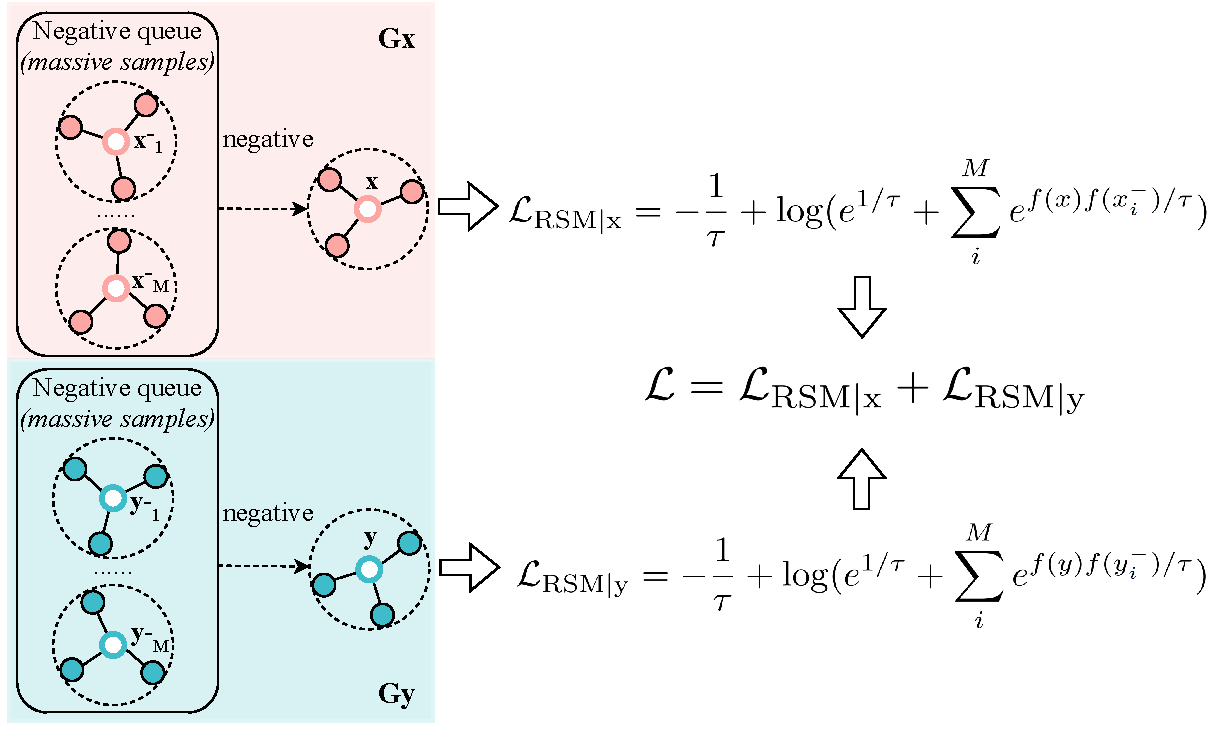
\includegraphics[width=0.99\columnwidth]{img/architecture_new3.pdf}
%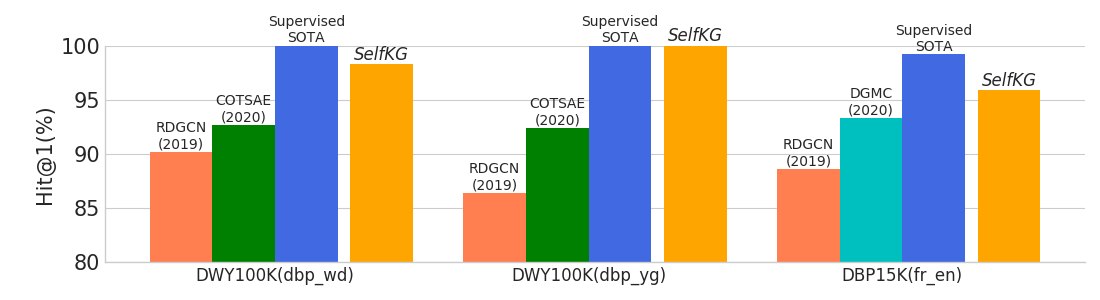
\includegraphics[width=1 \linewidth]{img/example.png}
\caption{The training process of \solution. 
\textmd{It leverages a negative queue for each KG to provide massive negative samples (up to 4k at a time) for calculating the self-supervised contrastive loss.}
}
\label{fig:modelflow}
\vspace{-3mm}
\end{figure}



%To deal with the expensive computational cost caused by 
%We introduce techniques in the next section to deal with the time complexity problem caused by a large number of negatives.

\subsection{Multiple Negative Queues}
\label{sec:mnq}

%~\cite{he2020momentum}.
Enlarging the number of negative samples can naturally result in additional computational cost, as  encoding massive negative samples on the fly is quite expensive. 
To address this issue, we propose to extend the MoCo technique~\cite{he2020momentum} for \solution. 
In Moco, a negative queue is maintained to store the previously-encoded batches as the encoded negative samples, which host thousands of encoded negative samples at limited cost. 

To adapt to the self-negative sampling strategy in \solution, we practically maintain two negative queues, associating with the two input KGs, respectively. 
An illustrative example is shown in Figure \ref{fig:modelflow}. 
In the beginning, we would not implement the gradient update until one of the queues reaches the predefined length $1+K$ where `$1$' is for the current batch and $K$ is for the number of previous batches used as negative samples. 
Given $|E|$ as the number of entities in a KG, $K$, and the batch size $N$ are constraint by
\begin{equation}
    (1+K)\times N< \min(|E_x|,|E_y|), 
\end{equation}
it is guaranteed that we would not sample out entities in the current batch. 
As a result, the real number of negative samples used for the current batch is $(1 + K)\times N - 1$.



\vpara{Momentum update~\cite{he2020momentum}.} 
The main challenge brought by negative queues is the obsolete encoded samples, especially for those encoded at the early stage of training, during which the model parameters vary drastically. 
Thus, the end-to-end training, which only uses one frequently-updated encoder, may actually harm the training. 
To mitigate this, we adopt the momentum training strategy, which maintains two encoders---the online encoder and the target encoder. 
While the online encoder's parameter $\theta_\mathsf{online}$ is instantly updated with the backpropagation, the target encoder $\theta_\mathsf{target}$ for encoding the current batch and then pushing into the negative queue is asynchronously updated with momentum by:
\begin{equation}
\label{eq:momentum}
    \theta_\mathsf{target} \gets m\cdot\theta_\mathsf{target} + (1-m)\cdot\theta_\mathsf{online}, m\in [0,1)
\end{equation}
A proper momentum is not only important for steady training but may also influence the final performance by avoiding representation collapse (Cf. Figure~\ref{fig:size_study}). We present a series of related hyper-parameter studies in Section~\ref{sec:exp}.



\vpara{Summary.}
We present \solution for self-supervised entity alignment.
\hhy{
Figure \ref{fig:motivations} illustrates that: 1. relative similarity metric (RSM) pushes the non-aligned entities ($y_0^-$, $y_1^-$ and $y_2^-$) of $x$ far enough, instead of directly pulling underlyingly-aligned $y$ close to $x$ (labeled pairs), enabling learning without label supervision; 
2. self-negative sampling samples negative entities for $x$ from ${G_x}$ to avoid sampling the true $y$ as its negative. }
Figure \ref{fig:modelflow} illustrates the training of \solution. 
It leverages existing techniques---embeddings from pre-trained language models and neighborhood aggregator---to initialize entity embeddings into a uni-space.  
The technical contributions of \solution lie in:
\begin{enumerate}
    \item  the design of the self-supervised loss in Eq.~\ref{eq:rsm} enabled by our relative similarity metric (RSM) in KGs; 
    \item  the strategy of self-negative sampling that furthers Eq.~\ref{eq:rsm} into Eq.~\ref{eq:xy} to avoid false-negative samples; 
    \item the extension of MoCo~\cite{he2020momentum} to two negative queues to support an efficient usage of massive negative samples. 
\end{enumerate}
